\heading{数学物理方法（上）-第3次作业}

\begin{question}
找出下列两个函数的分支点，并讨论 \(z\) 绕一个分支点移动一周回到原处后函数值的变化。如果同时绕两个、三个、乃至更多个分支点一周，函数值又如何变化？欢迎有兴趣的同学做成动画展示。

\begin{enumerate}
  \item \(z + \sqrt{1 - z^3}\);
  \item \(\sqrt[3]{1 - z^3}\).
\end{enumerate}
\begin{solution}
\begin{enumerate}
  \item 根式 \(1-z^3=0\) 时，有 \(z=1,\omega , \omega^2\)，其中 \(\omega=\ee^{\frac{2\pi}{3} \ii}\)。接下来验证其是否为分支点，我们可以将原式改写为 \[
w=z+\sqrt{(1-z)(\omega-z)(\omega^2-z)}
\] 在 \(\omega^m \;(m=0,1,2)\) 处取一半径小于 \(1\) 的圆，若 \(z\) 绕 \(\omega^m\) 转过一圈，则 \(\Delta \arg(\omega^m - z) = 2\pi\)，其余两个因子 \(\Delta \arg (\omega^k-z) =0\;(k \neq m)\)，因此 \(\Delta \arg \sqrt{1-z^3}=\pi\)，故都无法回到起始值。因此 \(1,\omega,\omega^2\) 都是分支点。

根式 \(1-z^3=\infty\) 时，有 \(z=\infty\)，做变换 \(t=1/z\)，有 \[
w = \frac1t+\sqrt{1-\frac1{t^3}}=\frac1t + \sqrt{\frac{t^3-1}{t^3}}
\] 在0取一半径小于 \(1/2\) 的圆，若 \(t\) 绕 \(0\) 转过一圈，则 \(\Delta \arg t^3=6\pi\)，故 \(\Delta \arg \sqrt{(t^3-1)/t^3}=-3\pi\)，无法回到起始值。因此 \(\infty\) 也是分支点。

综上而言，上述表达式有 \(1,\omega,\omega^2,\infty\) 四个分支点。

\medskip

若同时绕两个分支点一周，则 \(1-z,\omega-z,\omega^2-z\) 三个因子中，有两个因子 \(\Delta \arg = 2\pi\)，因此有 \(\Delta \arg \sqrt{1-z^3} = 2\pi\)，故函数值不变。（若绕行的点包含 \(\infty\)，则可以等效为绕其余两个分支点反方向一周，上述论证同样有效。）

若同时绕三个分支点一周，则 \(1-z,\omega-z,\omega^2-z\) 三个因子都有 \(\Delta \arg = 2\pi\)，因此有 \(\Delta \arg \sqrt{1-z^3} = 3\pi\)，故函数值改变。（实际上绕三个分支点转一周等价于绕剩余一个分支点反向转一周，故函数值会改变。）

  \item 根式 \(1-z^3=0\) 时，有 \(z=1,\omega,\omega^2\)，其中 \(\omega = \ee^{\frac{2\pi}{3} \ii}\)。接下来验证其是否为分支点，我们可以将原式改写为 \[
w=\sqrt[3]{(1-z)(\omega-z)(\omega^2-z)}
\] 在 \(\omega^m \;(m=0,1,2)\) 处取一半径小于 \(1\) 的圆，若 \(z\) 绕 \(\omega^m\) 转过一圈，则 \(\Delta \arg(\omega^m - z) = 2\pi\)，其余两个因子 \(\Delta \arg (\omega^k-z) =0\;(k \neq m)\)，因此 \(\Delta \arg \sqrt[3]{1-z^3}=\frac{2\pi}{3}\)，故都无法回到起始值。因此 \(1,\omega,\omega^2\) 都是分支点。

根式 \(1-z^3=\infty\) 时，有 \(z=\infty\)，做变换 \(t=1/z\)，有 \[
w =\sqrt[3]{1-\frac1{t^3}}=\sqrt[3]{\frac{t^3-1}{t^3}}
\] 在0取一半径小于 \(1/2\) 的圆，若 \(t\) 绕 \(0\) 转过一圈，则 \(\Delta \arg t^3=6\pi\)，故 \(\Delta \arg \sqrt[3]{(t^3-1)/t^3}=-2\pi\)，可以回到起始值。因此 \(\infty\) 不是分支点。

综上而言，上述表达式有 \(1,\omega,\omega^2\) 三个分支点。

\medskip

若同时绕两个分支点一周，则 \(1-z,\omega-z,\omega^2-z\) 三个因子中，有两个因子 \(\Delta \arg = 2\pi\)，因此有 \(\Delta \arg \sqrt[3]{1-z^3} = \frac{4\pi}{3}\)，故函数值改变。

若同时绕三个分支点一周，则 \(1-z,\omega-z,\omega^2-z\) 三个因子都有 \(\Delta \arg = 2\pi\)，因此有 \(\Delta \arg \sqrt[3]{1-z^3} = 2\pi\)，故函数值不改变。
\end{enumerate}
\end{solution}
\end{question}

\begin{question}
规定 \(0 \le \arg z < 2 \pi\)，求 \(w = \sqrt{z}\) 在 \(z = -\ii\) 处的导数值。如果规定 \(-\pi \le \arg z < \pi\)，那么 \(w = \sqrt{z}\) 在 \(z = -\ii\) 处的导数值又是多少？
\begin{solution}
求导计算可以得到 \(\dv{w}{z}= \frac{1}{2\sqrt{z}}\)。若取 \(0\le \arg z < 2\pi\)，有 \(\arg (-\ii)=\frac{3\pi}{2}\)，因此有 \[
\left. \dv{w}{z} \right|_{-\ii}= \frac{1}{2 \ee^{\ii \frac{3\pi}{4}}} =-\frac{\sqrt{2}}{4} (1+\ii)
\] 若取 \(-\pi \le \arg z < \pi\)，则 \(\arg (-\ii)=-\frac{\pi}{2}\)，因此有 \[
\left. \dv{w}{z} \right|_{-\ii} =\frac{1}{2 \ee^{-\ii \frac{\pi}{4}}} = \frac{\sqrt{2}}{4}(1+\ii)
\]
\end{solution}
\end{question}

\begin{question}
已知多值函数 \(w = z \sqrt[3]{z-2}\)，作割线，规定在割线上岸宗量 \(z-2\) 的辐角为0，试求在割线下岸 \(z=3\) 处的 \(w\) 值。

\begin{center}
\begin{tikzpicture}[scale=0.8]
\draw[->] (-2,0) -- (5,0) node[right] {$x$};
\draw[->] (0,-2.2) -- (0,2.2) node[above] {$y$};
\foreach \x in {-1,0,1,2,3}
  \filldraw (\x,0) circle (2pt) node[below] {$\x$};
\node at (0,1) [left] {$i$};
\node at (0,-1) [left] {$-i$};
% Branch cut (red) from z=2 along positive real axis
\draw[red,thick] (2,0.1) -- (4.8,0.1);
\draw[red,thick] (2,-0.1) -- (4.8,-0.1);
\draw[red,thick] (2,0.1) arc (90:270:0.1);
\node[text=red,fill=white,inner sep=1pt] at (3.4,0.45) {割线};
\end{tikzpicture}
\end{center}

又问：这个多值函数有几个单值分支？求出在其他几个单值分支中割线下岸 \(z=3\) 处的 \(w\) 值。

若规定 \(w(1) = \frac12 - \ii \frac{\sqrt{3}}{2}\)，求这时 \(w(3)=?\) 这相当于上面哪个单值分支？
\begin{solution}
考察如图所示的路径，有 \(\Delta \arg(z-2)=2\pi\)，因此 \(\Delta \arg \sqrt[3]{z-2} = \frac{2\pi}{3}\)。所以有 \[
\arg \sqrt[3]{z-2}=0+\frac{2\pi}{3}=\frac{2\pi}{3}
\] 因此可以得到 \(\sqrt[3]{z-2}=\ee^{\ii \frac{2\pi}{3}} = -\frac12+\ii \frac{\sqrt{3}}{2}\)，\(w=-\frac32+\ii \frac{3\sqrt{3}}{2}\)。

这个多值函数有三个单值分支，在其余分支中，割线下岸的 \(w\) 值为 \[
w'=-\frac32-\ii \frac{3\sqrt{3}}{2}, \quad w''=3 .
\]

若规定 \(w(1)=\frac12-\ii \frac{\sqrt{3}}{2}\)，则有 \[
\arg \sqrt[3]{z-2}= \Delta \arg+\arg w(1) = \frac{\pi}{3} + \left(-\frac{\pi}{3}\right) = 0,
\] 因此有 \(w(3) = 3\) 对应的是 \(w''\) 所在的分支。

\begin{center}
\begin{tikzpicture}[scale=0.8]
\draw[->] (-2,0) -- (5,0) node[right] {$x$};
\draw[->] (0,-2.2) -- (0,2.2) node[above] {$y$};
\foreach \x in {-1,0,1,2,3}
  \filldraw (\x,0) circle (2pt) node[below] {$\x$};
\node at (0,1) [left] {$i$};
\node at (0,-1) [left] {$-i$};
% Branch cut (red) from z=2 along positive real axis
\draw[red,thick] (2,0.1) -- (4.8,0.1);
\draw[red,thick] (2,-0.1) -- (4.8,-0.1);
\draw[red,thick] (2,0.1) arc (90:270:0.1);
\node[text=red,fill=white,inner sep=1pt] at (3.4,0.45) {割线};

% Blue path: large arc from z=3 above, around through z=1, back to z=3 below
\draw[blue,thick,->] (3,0.1) .. controls (2,0.3) and (1,0.2) .. (1,0)
                         .. controls (1,-0.2) and (2,-0.3) .. (3,-0.1);\end{tikzpicture}
\end{center}
\end{solution}
\end{question}

\begin{question}
求下列多值函数在指定点 \(z = \ii, 1, -1, (1+\ii)\) 的全部可能取值：
\begin{enumerate}
  \item \((z)^{\ii}\);
  \item \(\ln(z^{\ii})\).
\end{enumerate}
\begin{solution}
\begin{enumerate}
  \item \(z^{\ii}=\ee^{\ii \ln z}= \ee^{\ii (\ln|z|+\ii \arg z)}=\ee^{-\arg z+\ii \ln|z|}\)，
\begin{enumerate}
    \item \(z=\ii\)，有 \(\arg \ii = \frac{\pi}{2} + 2k \pi, |\ii|=1\)，故 \(\ii^{\ii}=\ee^{-\pi/2-2k \pi},(k \in \mathbb{Z})\)；
    \item \(z=1\)，有 \(\arg 1=2k \pi, |1|=1\)，故 \(1^{\ii} = \ee^{-2k \pi},(k \in \mathbb{Z})\)；
    \item \(z=-1\)，有 \(\arg (-1)=2k \pi+\pi, |-1|=1\)，故 \((-1)^{\ii} = \ee^{-\pi-2k \pi},(k \in \mathbb{Z})\)；
    \item \(z=1+\ii\)，有 \(\arg (1+\ii)=2k \pi+\frac{\pi}{4}, |1+\ii|=\sqrt{2}\)，故
    \[
    (1+\ii)^{\ii}
    =\ee^{-\pi/4-2k\pi+\ii\ln\sqrt{2}},
    \qquad k\in\mathbb{Z}.
    \]
\end{enumerate}

  \item \(\ln(z^{\ii})=\ln(\ee^{\ii \ln z})=-\arg z+\ii \ln|z| + \ii \cdot 2 \pi q\)，
\begin{enumerate}
    \item \(z=\ii\)，有 \(\arg \ii = \frac{\pi}{2} + 2k \pi, |\ii|=1\)，故 \(\ln(\ii^{\ii})=-\frac{\pi}{2}-2k \pi+\ii \cdot 2q \pi,(k, q \in \mathbb{Z})\)；
    \item \(z=1\)，有 \(\arg 1=2k \pi, |1|=1\)，故 \(\ln(1^{\ii}) = -2k \pi+\ii \cdot 2q \pi,(k, q \in \mathbb{Z})\)；
    \item \(z=-1\)，有 \(\arg (-1)=2k \pi+\pi, |-1|=1\)，故 \(\ln((-1)^{\ii}) = -\pi-2k \pi + \ii \cdot 2q \pi,(k, q \in \mathbb{Z})\)；
    \item \(z=1+\ii\)，有 \(\arg (1+\ii)=2k \pi+\frac{\pi}{4}, |1+\ii|=\sqrt{2}\)，故
    \[
    \ln((1+\ii)^{\ii})
    =-\frac{\pi}{4}-2k\pi
      +\ii\bigl(\ln\sqrt{2}+2q\pi\bigr),
    \qquad k,q\in\mathbb{Z}.
    \]
\end{enumerate}
\end{enumerate}
\end{solution}
\end{question}

\begin{question}
已知 \(f(z) = \sqrt{1-4z^2} + \ln \frac{1+2z}{1-2z}\)，规定 \(f(0) = -1 + 4\pi \ii\)，求 \(f(3)\)。

\begin{enumerate}
  \item 若沿路径 \(C_1\) 从 \(z=0\) 点到达 \(z=3\) 点；

  \item 若沿路径 \(C_2\) 从 \(z=0\) 点到达 \(z=3\) 点。

\begin{center}
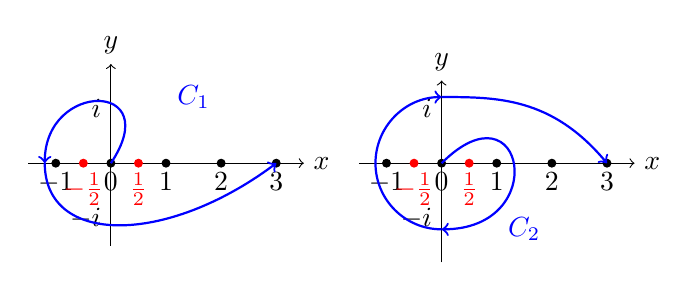
\begin{tikzpicture}[scale=0.7]
% Left figure: C1 path going above
\begin{scope}
\draw[->] (-1.5,0) -- (3.5,0) node[right] {$x$};
\draw[->] (0,-1.5) -- (0,1.8) node[above] {$y$};
\foreach \x in {-1,0,1,2,3}
  \filldraw (\x,0) circle (2pt) node[below] {$\x$};
\node at (0,1) [left] {$i$};
\node at (0,-1) [left] {$-i$};
% Branch points -1/2 and 1/2
\filldraw [red] (-0.5,0) circle (2pt) node[below] {$-\frac12$};
\filldraw [red] (0.5,0) circle (2pt) node[below] {$\frac12$};
% Path C1: exact Bezier curves from cetz
\draw[blue,thick,->] (0,0) .. controls (1,1.5) and (-1.2,1.5) .. (-1.2,0);
\draw[blue,thick,->] (-1.2,0) .. controls (-1.2,-1.5) and (1,-1.5) .. (3,0);
\node[text=blue,fill=white,inner sep=1pt] at (1.5,1.2) {$C_1$};
\end{scope}
% Right figure: C2 path
\begin{scope}[xshift=6cm]
\draw[->] (-1.5,0) -- (3.5,0) node[right] {$x$};
\draw[->] (0,-1.8) -- (0,1.5) node[above] {$y$};
\foreach \x in {-1,0,1,2,3}
  \filldraw (\x,0) circle (2pt) node[below] {$\x$};
\node at (0,1) [left] {$i$};
\node at (0,-1) [left] {$-i$};
% Branch points -1/2 and 1/2
\filldraw [red] (-0.5,0) circle (2pt) node[below] {$-\frac12$};
\filldraw [red] (0.5,0) circle (2pt) node[below] {$\frac12$};
% Path C2: exact Bezier curves from cetz
\draw[blue,thick,->] (0,0) .. controls (1.5,1.5) and (2,-1.2) .. (0,-1.2);
\draw[blue,thick,->] (0,-1.2) arc (-90:-270:1.2);
\draw[blue,thick,->] (0,1.2) .. controls (1,1.2) and (2,1.2) .. (3,0);
\node[text=blue,fill=white,inner sep=1pt] at (1.5,-1.2) {$C_2$};
\end{scope}
\end{tikzpicture}
\end{center}
\end{enumerate}
\begin{solution}
有 \(f(z)=\sqrt{(1-2z)(1+2z)} + \ln \frac{1+2z}{1-2z}\)，当 \(z=0\) 时，有 \(f(0)=\sqrt{1}+\ln 1=-1+4 \pi \ii\)，故在 \(z=0\) 处，可以设 \(\arg (1-4z^2)=2\pi, \arg \frac{1+2z}{1-2z}= 4\pi \)。

\begin{enumerate}
  \item 对于路径 \(C_1\)，有 \(\Delta \arg (\frac12-z)=\pi, \Delta \arg(\frac12+z)=2\pi\)，因此有 \[
\arg \sqrt{(1+2z)(1-2z)}=\frac{2\pi +2\pi + \pi}{2}= \frac52 \pi,
\quad \arg\frac{1+2z}{1-2z}=4\pi-\pi+2\pi=5\pi,
\] 故有 \(f(3)=\ln(7/5)+(\sqrt{35} + 5\pi) \ii\)。

  \item 对于路径 \(C_2\)，有 \(\Delta \arg(\frac12-z)=-3\pi, \Delta \arg(\frac12+z)=-2\pi\)，因此有 \[
\arg \sqrt{(1+2z)(1-2z)}=\frac{2\pi-3\pi-2\pi}{2}=-\frac32\pi,
\quad \arg\frac{1+2z}{1-2z}=4\pi+3\pi-2\pi=5\pi,
\] 故有 \(f(3)=\ln(7/5)+(\sqrt{35}+5\pi)\ii\)
\end{enumerate}
\end{solution}
\end{question}
\begin{question}
已知 \(w = \ln(1-z^2)\)，规定 \(w(0) = 0\)，试讨论当 \(z\) 限制在路径 (a) 和 (b) 中的 \(w(3)\) 值。若作割线 (c)，则在割线上、下岸 \(z=3\) 处 \(w\) 又取何值？

\begin{center}
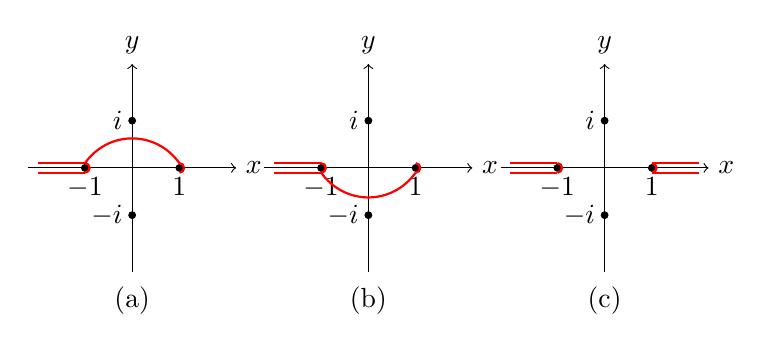
\begin{tikzpicture}[scale=0.6]
% (a)
\begin{scope}
\draw[->] (-2.2,0) -- (2.2,0) node[right] {$x$};
\draw[->] (0,-2.2) -- (0,2.2) node[above] {$y$};
\node at (-1,0) [below] {$-1$}; \node at (1,0) [below] {$1$};
\node at (0,1) [left] {$i$}; \node at (0,-1) [left] {$-i$};
\foreach \q in {(0,1),(0,-1),(-1,0),(1,0)} \filldraw \q circle (2pt);
\draw[red,thick] (1,-0.1) arc (-90:90:0.1);
\draw[red,thick] (1,0.1) .. controls (0.5,0.8) and (-0.5,0.8) .. (-1,0.1);
\draw[red,thick] (-1,0.1) -- (-2,0.1);
\draw[red,thick] (-2,-0.1) -- (-1,-0.1);
\draw[red,thick] (-1,-0.1) arc (-90:90:0.1);
\node at (0,-2.8) {(a)};
\end{scope}
% (b)
\begin{scope}[xshift=5cm]
\draw[->] (-2.2,0) -- (2.2,0) node[right] {$x$};
\draw[->] (0,-2.2) -- (0,2.2) node[above] {$y$};
\node at (-1,0) [below] {$-1$}; \node at (1,0) [below] {$1$};
\node at (0,1) [left] {$i$}; \node at (0,-1) [left] {$-i$};
\foreach \q in {(0,1),(0,-1),(-1,0),(1,0)} \filldraw \q circle (2pt);
\draw[red,thick] (1,0.1) arc (90:-90:0.1);
\draw[red,thick] (1,-0.1) .. controls (0.5,-0.8) and (-0.5,-0.8) .. (-1,-0.1);
\draw[red,thick] (-1,-0.1) -- (-2,-0.1);
\draw[red,thick] (-2,0.1) -- (-1,0.1);
\draw[red,thick] (-1,0.1) arc (90:-90:0.1);
\node at (0,-2.8) {(b)};
\end{scope}

% (c)
\begin{scope}[xshift=10cm]
\draw[->] (-2.2,0) -- (2.2,0) node[right] {$x$};
\draw[->] (0,-2.2) -- (0,2.2) node[above] {$y$};
\node at (-1,0) [below] {$-1$}; \node at (1,0) [below] {$1$};
\node at (0,1) [left] {$i$}; \node at (0,-1) [left] {$-i$};
\foreach \q in {(0,1),(0,-1),(-1,0),(1,0)} \filldraw \q circle (2pt);
\draw[red,thick] (-2,0.1) -- (-1,0.1);
\draw[red,thick] (-2,-0.1) -- (-1,-0.1);
\draw[red,thick] (-1,-0.1) arc (-90:90:0.1);
% Mirrored (right side)
\draw[red,thick] (2,0.1) -- (1,0.1);
\draw[red,thick] (2,-0.1) -- (1,-0.1);
\draw[red,thick] (1,-0.1) arc[start angle=-90, delta angle=180, radius=0.1];
\node at (0,-2.8) {(c)};
\end{scope}
\end{tikzpicture}
\end{center}

\begin{solution}

\begin{enumerate}
\item 由题，当 \(z=0\) 时，\(w=0\)，故 \(\bigl.\arg(1-z^2)\bigr|_{z=0}=0\)。考察路径 \(C_1\)，有
\[
\Delta\arg(1-z)=\pi,\quad \Delta\arg(1+z)=0,
\]
所以 \(\arg(1-z^2)=\pi\)，因此有
\[
w=\ln|1-z^2|+\ii\arg(1-z^2)=\ln 8+\pi\ii.
\]

\begin{center}
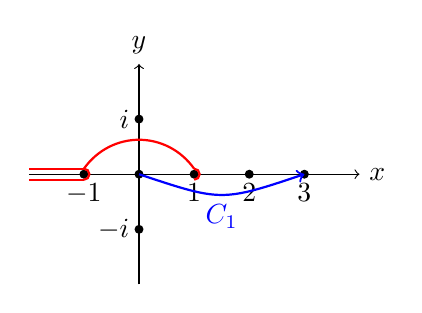
\begin{tikzpicture}[scale=0.7]
\draw[->] (-2,0) -- (4,0) node[right] {$x$};
\draw[->] (0,-2) -- (0,2) node[above] {$y$};
\node at (-1,0) [below] {$-1$}; \node at (1,0) [below] {$1$};
\node at (0,1) [left] {$i$}; \node at (0,-1) [left] {$-i$};
\foreach \x in {-1,1,0} \filldraw (\x,0) circle (2pt);
\foreach \y in {1,-1} \filldraw (0,\y) circle (2pt);
\foreach \i in {2,3} \filldraw (\i,0) circle (2pt) node[below] {$\i$};
\draw[red,thick] (1,-0.1) arc (-90:90:0.1);
\draw[red,thick] (1,0.1) .. controls (0.5,0.8) and (-0.5,0.8) .. (-1,0.1);
\draw[red,thick] (-1,0.1) -- (-2,0.1);
\draw[red,thick] (-2,-0.1) -- (-1,-0.1);
\draw[red,thick] (-1,-0.1) arc (-90:90:0.1);
\draw[blue,thick,->] (0,0) .. controls (1.5,-0.5) .. (3,0);
\node[text=blue,fill=white,inner sep=1pt,below] at (1.5,-0.5) {$C_1$};
\end{tikzpicture}
\end{center}

\item 由题，当 \(z=0\) 时，\(w=0\)，故 \(\bigl.\arg(1-z^2)\bigr|_{z=0}=0\)。考察路径 \(C_2\)，有
\[
\Delta\arg(1-z)=-\pi,\quad \Delta\arg(1+z)=0,
\]
所以 \(\arg(1-z^2)=-\pi\)，因此有
\[
w=\ln|1-z^2|+\ii\arg(1-z^2)=\ln 8-\pi\ii.
\]

\begin{center}
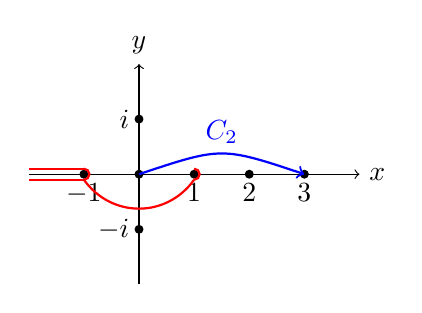
\begin{tikzpicture}[scale=0.7]
\draw[->] (-2,0) -- (4,0) node[right] {$x$};
\draw[->] (0,-2) -- (0,2) node[above] {$y$};
\node at (-1,0) [below] {$-1$}; \node at (1,0) [below] {$1$};
\node at (0,1) [left] {$i$}; \node at (0,-1) [left] {$-i$};
\foreach \x in {-1,1,0} \filldraw (\x,0) circle (2pt);
\foreach \y in {1,-1} \filldraw (0,\y) circle (2pt);
\foreach \i in {2,3} \filldraw (\i,0) circle (2pt) node[below] {$\i$};
\draw[red,thick] (1,0.1) arc (90:-90:0.1);
\draw[red,thick] (1,-0.1) .. controls (0.5,-0.8) and (-0.5,-0.8) .. (-1,-0.1);
\draw[red,thick] (-1,-0.1) -- (-2,-0.1);
\draw[red,thick] (-2,0.1) -- (-1,0.1);
\draw[red,thick] (-1,0.1) arc (90:-90:0.1);
\draw[blue,thick,->] (0,0) .. controls (1.5,0.5) .. (3,0);
\node[text=blue,fill=white,inner sep=1pt,above] at (1.5,0.5) {$C_2$};
\end{tikzpicture}
\end{center}

\item 沿着 \(C_1\) 可以走到割线下岸，即得到 \(w=\ln 8+\pi\ii\)；反之，沿着 \(C_2\) 可以走到割线上岸，即得到 \(w=\ln 8-\pi\ii\)。

\begin{center}
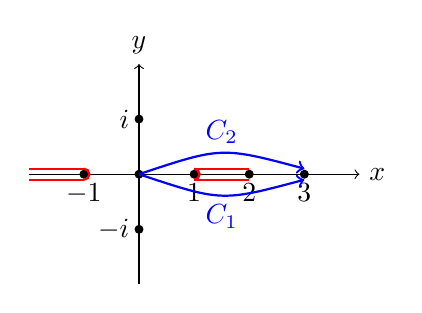
\begin{tikzpicture}[scale=0.7]
\draw[->] (-2,0) -- (4,0) node[right] {$x$};
\draw[->] (0,-2) -- (0,2) node[above] {$y$};
\node at (-1,0) [below] {$-1$}; \node at (1,0) [below] {$1$};
\node at (0,1) [left] {$i$}; \node at (0,-1) [left] {$-i$};
\foreach \x in {-1,1,0} \filldraw (\x,0) circle (2pt);
\foreach \y in {1,-1} \filldraw (0,\y) circle (2pt);
\foreach \i in {2,3} \filldraw (\i,0) circle (2pt) node[below] {$\i$};
\draw[blue,thick,->] (0,0) .. controls (1.5,-0.5) .. (3,-0.1);
\node[text=blue,fill=white,inner sep=1pt,below] at (1.5,-0.5) {$C_1$};
\draw[blue,thick,->] (0,0) .. controls (1.5,0.5) .. (3,0.1);
\node[text=blue,fill=white,inner sep=1pt,above] at (1.5,0.5) {$C_2$};
\draw[red,thick] (-2,0.1) -- (-1,0.1);
\draw[red,thick] (-2,-0.1) -- (-1,-0.1);
\draw[red,thick] (-1,-0.1) arc (-90:90:0.1);
% Mirrored (right side)
\draw[red,thick] (2,0.1) -- (1,0.1);
\draw[red,thick] (2,-0.1) -- (1,-0.1);
\draw[red,thick] (1,-0.1) arc[start angle=-90, delta angle=180, radius=0.1];
\end{tikzpicture}
\end{center}
\end{enumerate}

\end{solution}
\end{question}

\begin{question}
反正切 \(\arctan z\) 的定义为
\[
\arctan z = \frac{1}{2\ii}\ln\frac{1+\ii z}{1-\ii z}.
\]
若作割线，并规定
\[
\bigl.\arctan z\bigr|_{z=0} = \pi,
\]
求函数在 \(z=2\) 处的函数值和导数值。此时当 \(z\to\infty\) 时，\(\arctan z\) 的极限存在吗？若存在，极限值是多少？
如果换一种割线作法，沿虚轴连接 \(z=\ii\) 和 \(z=-\ii\) 作割线，规定函数在 \(z=2\) 处的函数值为上面求到的值，新的割线作法下，当 \(z\to\infty\) 时，\(\arctan z\) 的极限存在吗？若存在，极限值是多少？

\begin{center}
\begin{tikzpicture}[scale=1.2]
\draw[->] (-1.5,0) -- (2,0) node[right] {$x$};
\draw[->] (0,-3) -- (0,3) node[above] {$y$};
\foreach \x in {-1,1} \filldraw (\x,0) circle (2pt) node[below] {$\x$};
\filldraw (0,1) circle (2pt) node[right] {$\ii$};
\filldraw (0,-1) circle (2pt) node[right] {$-\ii$};
% Lower branch cut (from -i down)
\draw[red,thick] (0.1,-1) -- (0.1,-3);
\draw[red,thick] (-0.1,-1) -- (-0.1,-3);
\draw[red,thick] (0.1,-1) arc (0:180:0.1);
% Upper branch cut (from i up, mirrored by rotate x: 180deg)
\draw[red,thick] (0.1,1) -- (0.1,3);
\draw[red,thick] (-0.1,1) -- (-0.1,3);
\draw[red,thick] (0.1,1) arc (0:-180:0.1);
\end{tikzpicture}
\end{center}

\begin{solution}
有 \(\arctan z = \dfrac{1}{2\ii}\ln\dfrac{\ii-z}{\ii+z}\)，由 \(\bigl.\arctan z\bigr|_{z=0}=\pi\)，则 \(\bigl.\arg\dfrac{\ii-z}{\ii+z}\bigr|_{z=0}=2\pi\)。考察由 \(0\) 到 \(2\) 的一条直线，有
\[
\Delta\arg(\ii-z)=\arctan 2,\quad \Delta\arg(\ii+z)=-\arctan 2,
\]
因此
\[
\bigl.\arg\frac{\ii-z}{\ii+z}\bigr|_{z=2}=2\pi+2\arctan 2,
\]
故 \(\bigl.\arctan z\bigr|_{z=2}=\pi+\arctan 2\)。而 \((\arctan z)'=\dfrac{1}{1+z^2}\)，当 \(z=2\) 时，导数为 \(\dfrac15\)。

为了考察 \(\infty\) 处 \(\arctan z\) 的极限，做变换 \(t=1/z\)，有 \(\arctan(1/t)=\dfrac{1}{2\ii}\ln\dfrac{t+\ii}{t-\ii}\)。在 \(t\) 平面上，割线变为沿虚轴连接 \(\ii\) 到 \(-\ii\) 的线段。在割线两侧 \(t=0\) 处的取值不相等，故极限不存在。

若更换割线做法，在 \(t\) 平面上，割线变为沿虚轴连接 \(\ii\) 到 \(\infty\)，再由 \(\infty\) 连接到 \(-\ii\) 的两段射线。割线不经过 \(t=0\) 处，故极限存在。考察由 \(t=1/2\) 到 \(t=0\) 的直线段，有
\[
\bigl.\arg\frac{t+\ii}{t-\ii}\bigr|_{t=1/2}=2\pi+2\arctan 2,\quad
\Delta\arg(t+\ii)=\arctan\frac12,\quad
\Delta\arg(t-\ii)=-\arctan\frac12,
\]
因此可以得到
\[
\bigl.\arg\frac{t+\ii}{t-\ii}\bigr|_{t=0}=3\pi,
\]
故 \(\displaystyle\lim_{z\to\infty}\arctan z=\frac{3\pi}{2}\)。
\end{solution}
\end{question}

\begin{question}
试按给定的路径计算下列积分：
\[
\int_C\frac{\dd{z}}{\sqrt{z}},
\]
规定 \(\sqrt{1}=1\)，积分路径为由 \(z=1\) 出发的：
\begin{enumerate}
  \item 单位圆的上半周；
  \item 单位圆的下半周。
\end{enumerate}
\begin{solution}
设 \(z=\ee^{\ii\theta}\)，则
\[
\frac{\dd{z}}{\sqrt z}
=\ii\ee^{\ii\theta}\ee^{-\ii\theta/2}\dd{\theta}
=\ii\ee^{\ii\theta/2}\dd{\theta}.
\]

\begin{enumerate}
  \item
  \[
  I_1=\int_0^\pi\ii\ee^{\ii\theta/2}\dd{\theta}
  =\left.2\ee^{\ii\theta/2}\right|_0^\pi
  =2\ii-2.
  \]
  \item
  \[
  I_2=\int_0^{-\pi}\ii\ee^{\ii\theta/2}\dd{\theta}
  =\left.2\ee^{\ii\theta/2}\right|_0^{-\pi}
  =-2\ii-2.
  \]
\end{enumerate}
\end{solution}
\end{question}

\begin{question}
计算下列积分：
\begin{enumerate}
  \item \(\displaystyle\int_C\operatorname{Im}z\,\dd{z},\)
  \item \(\displaystyle\int_C|\operatorname{Im}z|\,\dd{z},\)
  \item \(\displaystyle\int_C\operatorname{Im}z\,|\dd{z}|,\)
  \item \(\displaystyle\int_C|\operatorname{Im}z|\,|\dd{z}|,\)
\end{enumerate}
其中 \(C\) 为从复数 \(-1-\ii\) 到 \(1-\ii\) 再到 \(1+\ii\) 的折线。

\begin{center}
\begin{tikzpicture}[scale=1.2]
\draw[->] (-2,0) -- (2,0) node[right] {$x$};
\draw[->] (0,-2) -- (0,2) node[above] {$y$};
\draw[thick] (-1,-1) -- (1,-1) -- (1,1);
\filldraw (-1,-1) circle (2pt) node[above right] {$-1-\ii$};
\filldraw (1,-1) circle (2pt) node[above] {$1-\ii$};
\filldraw (1,1) circle (2pt) node[right] {$1+\ii$};
\node at (0,0) [below left] {$O$};
\end{tikzpicture}
\end{center}

\begin{solution}
\begin{enumerate}
  \item
  \[
  I_1=\int_{-1}^{1}(-1)\dd{x}
  +\ii\int_{-1}^{1}y\dd{y}
  =-2.
  \]
  \item \(\displaystyle I_2=\int_{-1}^{1}1\,\dd{x}+\int_{-1}^{1}|y|\,\ii\,\dd{y}=2+\ii\)。
  \item
  \[
  I_3=\int_{-1}^{1}(-1)\dd{x}
  +\int_{-1}^{1}y\dd{y}
  =-2.
  \]
    \item \(\displaystyle I_4=\int_{-1}^{1}1\,\dd{x}+\int_{-1}^{1}|y|\,\dd{y}=2+2\int_{0}^{1}y\,\dd{y}=3\)。
  \end{enumerate}
  \end{solution}
  \end{question}
